% Options for packages loaded elsewhere
\PassOptionsToPackage{unicode}{hyperref}
\PassOptionsToPackage{hyphens}{url}
\PassOptionsToPackage{dvipsnames,svgnames,x11names}{xcolor}
%
\documentclass[
  11pt,
]{book}
\usepackage{amsmath,amssymb}
\usepackage{lmodern}
\usepackage{iftex}
\ifPDFTeX
  \usepackage[T1]{fontenc}
  \usepackage[utf8]{inputenc}
  \usepackage{textcomp} % provide euro and other symbols
\else % if luatex or xetex
  \usepackage{unicode-math}
  \defaultfontfeatures{Scale=MatchLowercase}
  \defaultfontfeatures[\rmfamily]{Ligatures=TeX,Scale=1}
\fi
% Use upquote if available, for straight quotes in verbatim environments
\IfFileExists{upquote.sty}{\usepackage{upquote}}{}
\IfFileExists{microtype.sty}{% use microtype if available
  \usepackage[]{microtype}
  \UseMicrotypeSet[protrusion]{basicmath} % disable protrusion for tt fonts
}{}
\makeatletter
\@ifundefined{KOMAClassName}{% if non-KOMA class
  \IfFileExists{parskip.sty}{%
    \usepackage{parskip}
  }{% else
    \setlength{\parindent}{0pt}
    \setlength{\parskip}{6pt plus 2pt minus 1pt}}
}{% if KOMA class
  \KOMAoptions{parskip=half}}
\makeatother
\usepackage{xcolor}
\IfFileExists{xurl.sty}{\usepackage{xurl}}{} % add URL line breaks if available
\IfFileExists{bookmark.sty}{\usepackage{bookmark}}{\usepackage{hyperref}}
\hypersetup{
  pdftitle={Risk Analysis in the Earth Sciences},
  pdfauthor={Vivek Srikrishnan; Klaus Keller},
  colorlinks=true,
  linkcolor={Maroon},
  filecolor={Maroon},
  citecolor={Blue},
  urlcolor={Blue},
  pdfcreator={LaTeX via pandoc}}
\urlstyle{same} % disable monospaced font for URLs
\usepackage{color}
\usepackage{fancyvrb}
\newcommand{\VerbBar}{|}
\newcommand{\VERB}{\Verb[commandchars=\\\{\}]}
\DefineVerbatimEnvironment{Highlighting}{Verbatim}{commandchars=\\\{\}}
% Add ',fontsize=\small' for more characters per line
\usepackage{framed}
\definecolor{shadecolor}{RGB}{248,248,248}
\newenvironment{Shaded}{\begin{snugshade}}{\end{snugshade}}
\newcommand{\AlertTok}[1]{\textcolor[rgb]{0.33,0.33,0.33}{#1}}
\newcommand{\AnnotationTok}[1]{\textcolor[rgb]{0.37,0.37,0.37}{\textbf{\textit{#1}}}}
\newcommand{\AttributeTok}[1]{\textcolor[rgb]{0.61,0.61,0.61}{#1}}
\newcommand{\BaseNTok}[1]{\textcolor[rgb]{0.06,0.06,0.06}{#1}}
\newcommand{\BuiltInTok}[1]{#1}
\newcommand{\CharTok}[1]{\textcolor[rgb]{0.5,0.5,0.5}{#1}}
\newcommand{\CommentTok}[1]{\textcolor[rgb]{0.37,0.37,0.37}{\textit{#1}}}
\newcommand{\CommentVarTok}[1]{\textcolor[rgb]{0.37,0.37,0.37}{\textbf{\textit{#1}}}}
\newcommand{\ConstantTok}[1]{\textcolor[rgb]{0,0,0}{#1}}
\newcommand{\ControlFlowTok}[1]{\textcolor[rgb]{0.27,0.27,0.27}{\textbf{#1}}}
\newcommand{\DataTypeTok}[1]{\textcolor[rgb]{0.27,0.27,0.27}{#1}}
\newcommand{\DecValTok}[1]{\textcolor[rgb]{0.06,0.06,0.06}{#1}}
\newcommand{\DocumentationTok}[1]{\textcolor[rgb]{0.37,0.37,0.37}{\textbf{\textit{#1}}}}
\newcommand{\ErrorTok}[1]{\textcolor[rgb]{0.14,0.14,0.14}{\textbf{#1}}}
\newcommand{\ExtensionTok}[1]{#1}
\newcommand{\FloatTok}[1]{\textcolor[rgb]{0.06,0.06,0.06}{#1}}
\newcommand{\FunctionTok}[1]{\textcolor[rgb]{0,0,0}{#1}}
\newcommand{\ImportTok}[1]{#1}
\newcommand{\InformationTok}[1]{\textcolor[rgb]{0.37,0.37,0.37}{\textbf{\textit{#1}}}}
\newcommand{\KeywordTok}[1]{\textcolor[rgb]{0.27,0.27,0.27}{\textbf{#1}}}
\newcommand{\NormalTok}[1]{#1}
\newcommand{\OperatorTok}[1]{\textcolor[rgb]{0.43,0.43,0.43}{\textbf{#1}}}
\newcommand{\OtherTok}[1]{\textcolor[rgb]{0.37,0.37,0.37}{#1}}
\newcommand{\PreprocessorTok}[1]{\textcolor[rgb]{0.37,0.37,0.37}{\textit{#1}}}
\newcommand{\RegionMarkerTok}[1]{#1}
\newcommand{\SpecialCharTok}[1]{\textcolor[rgb]{0,0,0}{#1}}
\newcommand{\SpecialStringTok}[1]{\textcolor[rgb]{0.5,0.5,0.5}{#1}}
\newcommand{\StringTok}[1]{\textcolor[rgb]{0.5,0.5,0.5}{#1}}
\newcommand{\VariableTok}[1]{\textcolor[rgb]{0,0,0}{#1}}
\newcommand{\VerbatimStringTok}[1]{\textcolor[rgb]{0.5,0.5,0.5}{#1}}
\newcommand{\WarningTok}[1]{\textcolor[rgb]{0.37,0.37,0.37}{\textbf{\textit{#1}}}}
\usepackage{longtable,booktabs,array}
\usepackage{calc} % for calculating minipage widths
% Correct order of tables after \paragraph or \subparagraph
\usepackage{etoolbox}
\makeatletter
\patchcmd\longtable{\par}{\if@noskipsec\mbox{}\fi\par}{}{}
\makeatother
% Allow footnotes in longtable head/foot
\IfFileExists{footnotehyper.sty}{\usepackage{footnotehyper}}{\usepackage{footnote}}
\makesavenoteenv{longtable}
\usepackage{graphicx}
\makeatletter
\def\maxwidth{\ifdim\Gin@nat@width>\linewidth\linewidth\else\Gin@nat@width\fi}
\def\maxheight{\ifdim\Gin@nat@height>\textheight\textheight\else\Gin@nat@height\fi}
\makeatother
% Scale images if necessary, so that they will not overflow the page
% margins by default, and it is still possible to overwrite the defaults
% using explicit options in \includegraphics[width, height, ...]{}
\setkeys{Gin}{width=\maxwidth,height=\maxheight,keepaspectratio}
% Set default figure placement to htbp
\makeatletter
\def\fps@figure{htbp}
\makeatother
\setlength{\emergencystretch}{3em} % prevent overfull lines
\providecommand{\tightlist}{%
  \setlength{\itemsep}{0pt}\setlength{\parskip}{0pt}}
\setcounter{secnumdepth}{5}
\usepackage{tcolorbox}

\newtcolorbox{info}{title=Info, colback=blue!5, colframe=blue!75!black}
\newtcolorbox{warning}{title=Warning, colback=red!5, colframe=red!75!black}

\usepackage{afterpage}
\usepackage{geometry}
\usepackage{csquotes}

%\usepackage{FiraMono}
%\usepackage[sfdefault]{FiraSans} %% option 'sfdefault' activates Fira Sans as the default text font
%\usepackage[T1]{fontenc}
%\renewcommand*\oldstylenums[1]{{\firaoldstyle #1}}

% \setmonofont[
%     Extension   = .otf,
%     UprightFont = *-Regular,
%     BoldFont    = *-Medium
% ]{FiraMono}

%\setsansfont[
%    Extension      = .otf,
%    UprightFont    = *-Light,
%    ItalicFont     = *-LightItalic,
%    BoldFont       = *-Regular
%]{FiraSans}

\frontmatter
\ifLuaTeX
  \usepackage{selnolig}  % disable illegal ligatures
\fi
\usepackage[]{natbib}
\bibliographystyle{plainnat}

\title{Risk Analysis in the Earth Sciences}
\author{Vivek Srikrishnan\footnote{Department of Biological \& Environmental Engineering, Cornell University, \href{mailto:viveks@cornell.edu}{\nolinkurl{viveks@cornell.edu}}} \and Klaus Keller\footnote{Thayer School of Engineering, Dartmouth University, \href{mailto:klaus.keller@dartmouth.edu}{\nolinkurl{klaus.keller@dartmouth.edu}}}}
\date{2021-12-05}

\begin{document}




\newgeometry{margin=0.35in}  
\begin{center}
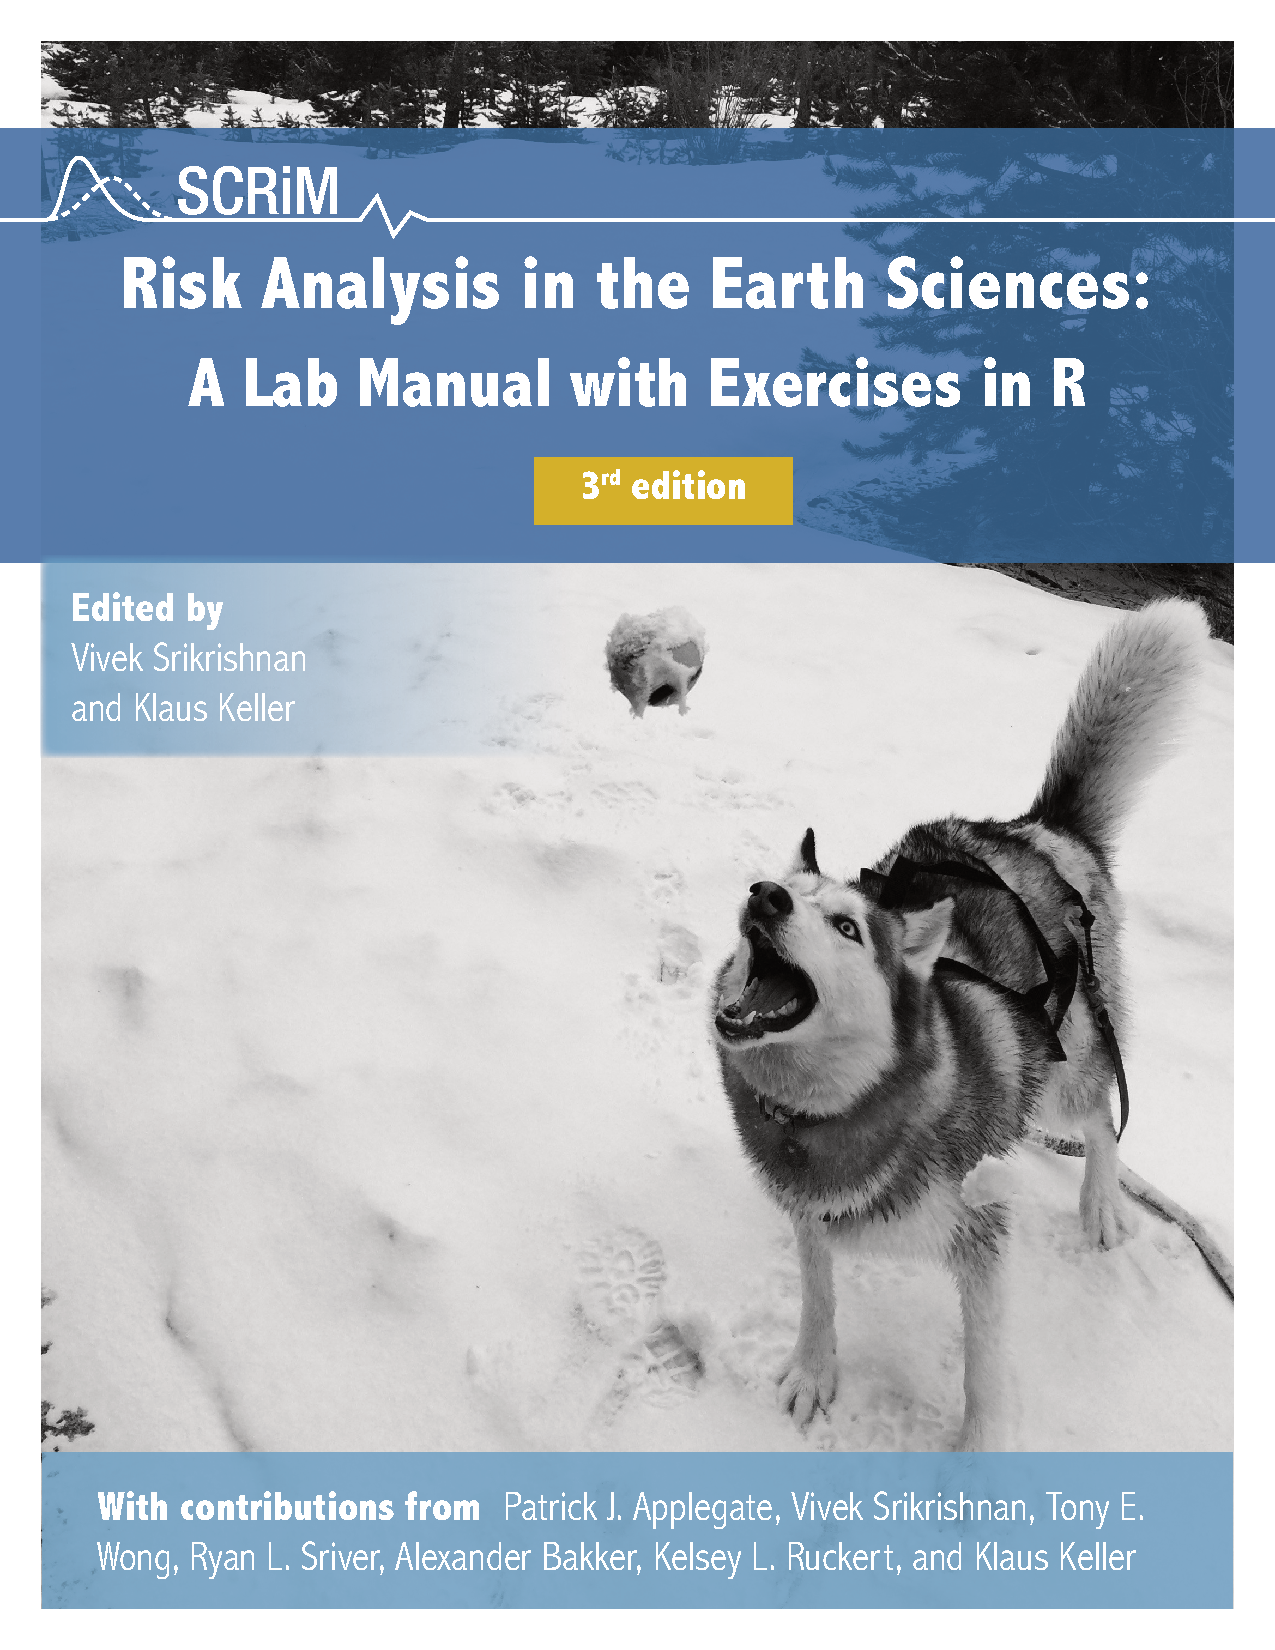
\includegraphics{images/cover_with_alexander.pdf}
\end{center}
\thispagestyle{empty}

\clearpage

\restoregeometry


\maketitle


{
\hypersetup{linkcolor=}
\setcounter{tocdepth}{2}
\tableofcontents
}
\hypertarget{preface}{%
\chapter*{Preface}\label{preface}}


Greenhouse gas emissions have caused considerable changes in climate, including increased surface air temperatures and rising sea levels. Rising sea levels increase the risks of flooding for people living near the world's coastlines. Managing such risks requires an understanding of many fields, including Earth science, statistics, and economics. At the same time, the free, open-source programming environment \href{http://www.julialang.org}{Julia} is growing in popularity among statisticians and scientists due to its flexibility and graphics capabilities, as well as its large collection of existing software libraries.

This textbook presents a series of exercises in Julia that teach the Earth science and statistical concepts needed for assessing climate-related risks. These exercises are intended for upper-level undergraduates, beginning graduate students, and professionals in other areas who wish to gain insight into academic climate risk analysis.

The content of this book is licensed under the \href{https://creativecommons.org/licenses/by-nc-sa/4.0/}{Creative Commons Attribution-NonCommercial-ShareAlike 4.0 International License}.

\hypertarget{about-this-book}{%
\chapter*{About This Book}\label{about-this-book}}


This textbook presents a series of chapters that introduce students to the statistical aspects of risk analysis in the Earth sciences using Julia. Most of these chapters have to do with sea-level rise, which is a major focus of the authors' research activities.

The exercises are intended for upper-level undergraduates, beginning graduate students, and professionals in other areas who wish to gain insight into academic climate risk analysis. Previous programming experience is helpful, but not required; the first exercise explains how to learn the basics of Julia.

Each chapter begins with a description of the Earth science and/or statistical concepts that the chapter teaches. Next, each chapter presents a detailed explanation of a piece of existing Julia code. Finally, students are asked to either modify the existing code or write their own code to produce a well-defined outcome. Each chapter also includes questions to encourage classroom discussion and reflection on the part of individual students.

A few chapters contain appendices that present additional discussion of the topics raised in the preceding parts of those chapters. These appendices are intended for graduate students or researchers who have additional background in programming or the Earth sciences. They can be skipped by other readers with no loss in comprehension.

The book is designed to be modular. The first eight chapters (0-7) were written by Patrick Applegate, with contributions by others as noted in the individual chapters. Chapter 8 was written by Vivek Srikrishnan, and Chapter 9 by Tony Wong. Other chapters may be added by members of the Keller research group in the future.

\begin{center}

\begin{warning}
Completing the chapters in this textbook will not teach you to perform publication-quality or consulting-grade risk analyses. This textbook is intended primarily for advanced undergraduates, and the material presented here should only be applied to \enquote{real} problems after additional training. The authors and editors of this textbook specifically disclaim any liability for damages associated with the use of the material presented in this textbook.

\end{warning}


\end{center}

\hypertarget{contributor-bios}{%
\section*{Contributor Bios}\label{contributor-bios}}


\textbf{Vivek Srikrishnan} is an Assistant Professor in the Department of Biological \& Environmental Engineering at Cornell University. He studies decision-making under uncertain climate risks and feedbacks between natural and human systems. His research combines model development, uncertainty quantification, complex systems dynamics, and decision-making under uncertainty. He has a Ph.D.~in Energy \& Mineral Engineering from Penn State. Vivek's email address is \href{mailto:viveks@cornell.edu}{\nolinkurl{viveks@cornell.edu}}, and his website is \url{http://www.viveks.me}.

\textbf{Patrick J. Applegate} is an Academic Editor at Research Square. In this role, Patrick helps researchers communicate their science and works on data science projects in Python. Patrick earned his Ph.D.~in Geosciences at Penn State and is first author or co-author of 20 peer-reviewed scientific papers. His research treats topics including ice sheets and their contributions to sea level rise, methods for estimating the ages of glacial deposits, and the application of statistical methods to problems in the geosciences.

\textbf{Tony E. Wong} is an Assistant Professor in the School of Mathematical \& Statistical Sciences at the Rochester Institute of Technology. He received his PhD in Applied Mathematics from CU Boulder in 2016, and later was a Postdoctoral Scholar at Penn State's Earth and Environmental Systems Institute. Prior to joining RIT, Tony returned to CU as an Instructor in the Department of Computer Science to pursue his love of teaching. His current research focuses on uncertainty quantification and model calibration in sea level and coastal storm surge projections. Tony's email address is \href{mailto:aeswma@rit.edu}{\nolinkurl{aeswma@rit.edu}} and his website is \url{https://tonyewong.github.io}.

\textbf{Ryan L. Sriver} is an Associate Professor of Atmospheric Sciences at the University of Illinois at Urbana-Champaign (UIUC). Prior to joining UIUC in the fall of 2012, he worked as a research associate in Penn State's Department of Geosciences and as a NOAA Climate and Global Change postdoctoral fellow in Penn State's Department of Meteorology. He graduated from Purdue University with a Ph.D.~in Earth and Atmospheric Sciences. His research seeks to develop a deeper understanding about the physical processes influencing variability within Earth's climate system, and to quantify climate change uncertainties relevant to adaptation planning and decision-making. Ryan's email address is \href{mailto:rsriver@illinois.edu}{\nolinkurl{rsriver@illinois.edu}}, and his website is at \url{https://www.atmos.illinois.edu/~rsriver/index.html}.

\textbf{Alexander Bakker} is a senior advisor at Rijkswaterstraat. He received a Masters in Civil Engineering from the Delft University of Technology and obtained a PhD in Regional climate change scenarios at VU University of Amsterdam.

\textbf{Kelsey L. Ruckert} is a geologist by training. She is a Coastal Extension Specialist for the Earth and Environmental Systems Institute at Penn State. She specializes in geology, flood hazards, water quality, and climate change impacts where she excels in GIS, statistical analysis, modeling, and fieldwork. Her research focuses on understanding sea-level rise, storm surge, and water resources, and their implications to vulnerability and the design of risk management strategies. Her email address is \href{mailto:klr324@psu.edu}{\nolinkurl{klr324@psu.edu}} and her website is \url{http://klr324.github.io}.

\textbf{Klaus Keller} is a Professor of Geosciences at Penn State and a Visiting Professor at the Thayer School of Engineering at Dartmouth University. Keller directs the Center for Climate Risk Management as well as the research network for \href{https://scrimhub.org}{Sustainable Climate Risk Management}. Before joining Penn State, he worked as a research scientist and lecturer at Princeton University and as an engineer in Germany. Professor Keller graduated from Princeton with a Ph.D.~in civil and environmental engineering. He received master's degrees from M.I.T. and Princeton as well as an engineer's degree from the Technische Universität Berlin. His research addresses two interrelated questions. First, how can we mechanistically understand past and potentially predict future changes in the climate system? Second, how can we use this information to design sustainable, scientifically sound, technologically feasible, economically efficient, and ethically defensible climate risk management strategies? He analyzes these questions by mission-oriented basic research covering a wide range of disciplines such as Earth system science, economics, engineering, philosophy, decision science, and statistics. Klaus' email address is \href{mailto:klaus@psu.edu}{\nolinkurl{klaus@psu.edu}}, and website is at \url{http://www3.geosc.psu.edu/~kzk10/}.

\hypertarget{acknowledgements}{%
\section*{Acknowledgements}\label{acknowledgements}}


This work was supported by the National Science Foundation through the Network for Sustainable Climate Risk Management (SCRiM) under NSF cooperative agreement GEO-1240507. Any opinions, findings, and conclusions or recommendations expressed in this material are those of the author(s) and do not necessarily reflect the views of the National Science Foundation. Other support was provided by the \href{http://www.clima.psu.edu/index.php}{Center for Climate Risk Management} and the \href{http://rockethics.psu.edu}{Rock Ethics Institute}.

Most of these exercises were originally developed as part of a course titled \href{http://bulletins.psu.edu/undergrad/courses/G/GEOSC/450/200910SP}{Risk Analysis in the Earth Sciences}, developed and taught by Klaus Keller in the \href{http://www.geosc.psu.edu}{Department of Geosciences} at the \href{http://www.psu.edu}{Pennsylvania State University}. The exercises discussed in this lab manual were co-developed by a large group (see the individual chapters).

Katerina Kostadinova designed the cover using a photograph provided by Frank Erickson.

Randy Miller created the Github repository.

Thomas Patrick Walsh and Naomi Radke made suggestions for improving the text and lab exercises.

\textbf{Vivek Srikrishnan} thanks his colleagues in the Keller research group and beyond for being willing and able to work on this textbook. Special thanks go to Patrick Applegate for leading the development of an excellent first edition of this book.

\textbf{Klaus Keller} thanks all the students from the Risk Analysis course, the members of the Keller research group, and his SCRiM collaborators for invaluable inputs. Special thanks go to his family, many mentors, and friends for support.

\hypertarget{book-source-and-scripts}{%
\section*{Book Source and Scripts}\label{book-source-and-scripts}}


As noted above, most of the exercises presented in this e-textbook ask students to modify existing R scripts. These R scripts can be downloaded as a \texttt{.zip} file from \url{https://www.scrimhub.org/raes}.

The source files for the book are stored in a Github repository at \url{https://github.com/scrim-network/raes}.

\hypertarget{comments-and-questions}{%
\section*{Comments and Questions}\label{comments-and-questions}}


We'd like to make \emph{Risk Analysis in the Earth Sciences} as useful as possible. If you have a comment about the book or a question about one of the chapters, please post an issue to the \href{https://github.com/scrim-network/raes}{Github repository} mentioned above. If we make a change to the book based on your comments, we will be sure to add your name to the Acknowledgements section in future versions.

\mainmatter

\hypertarget{introduction}{%
\chapter{Introduction}\label{introduction}}

This chapter was written by Patrick J. Applegate and Klaus Keller. It briefly discusses climate change, uncertainty, and risk.

\hypertarget{climate-risks}{%
\section{Climate Risks}\label{climate-risks}}

We begin with a very brief discussion of some key findings of climate science and the problems posed by climate change. There are many useful reviews of these subjects, in both textbook and popular formats \citep{Kump2009-no, Alley2011-by}. For high-level discussions of these topics, see the \href{http://www.ipcc.ch/index.htm}{Intergovernmental Panel on Climate Change}'s recent reports, particularly the Technical Summaries of the IPCC's Working Groups I and II \citep{Stocker2013-am, Field2013-pl}. We particularly recommend that you read chapters 1, 3, 6, 15, and 16 in \citet{Kump2009-no} before working on the exercises in this e-textbook.

Most scientists who study the climate system agree that human activities are causing surface air temperatures to increase \citep{Oreskes2007-fj}. Combustion of fossil fuels and changes in land use lead to increases in the concentrations of carbon dioxide, methane, and nitrous oxide in the atmosphere. The increased concentrations of these gases trap heat near the earth's surface that would normally escape to outer space. Temperatures have risen measurably over the last century and will probably continue to increase in the future \citep{Ipcc2013-px, Collins2013-yi}.

This increase in surface air temperatures affects other parts of the Earth system, notably sea level. Rising surface air temperatures cause the water near the ocean's surface to expand, and also lead to increased rates of melting from land ice. Global mean sea level has risen by a few tens of centimeters over the past 1-2 centuries, and could go up by more than one meter by 2100 \citep{Parris2012-qw, Ipcc2013-px, Church2013-el}.

Increases in sea level create risks for people living near present-day sea level. Sea level at a particular point along the world's coastline rises and falls over time scales of hours to days, in response to tides and storms. Stacked on top of the long-term rise in sea level, these short-period oscillations flood normally-dry land with increased frequency \citep[e.g.~][]{Spanger-Siegfried2014-mx}.

Fossil fuel consumption also creates benefits for people, although these benefits are unevenly distributed. Countries with low per capita \href{https://en.wikipedia.org/wiki/Gross_domestic_product}{gross domestic products} also tend to emit very little carbon dioxide per person. Among countries with high per capita gross domestic products, some emit large amounts of carbon dioxide per person each year, whereas others emit comparatively little. However, achieving good economic outcomes in today's energy economy seems to require at least some fossil fuel consumption. Moreover, the benefits of fossil fuel consumption occur now, whereas the negative effects of climate change will take place primarily in the future.

Thus, reducing greenhouse gas emissions creates costs in terms of lost economic productivity. Modern societies require large amounts of energy to manufacture goods, produce food, and move people from place to place. Today, \href{https://www.iea.org/fuels-and-technologies}{most of that energy comes from fossil fuels}. Reducing fossil fuel consumption likely means cuts to manufacturing, agriculture, or transportation, at least in the short term.

\hypertarget{some-questions}{%
\section{Some Questions}\label{some-questions}}

The discussion in Chapter \ref{climate-risks} leads to several interrelated questions:

\begin{enumerate}
\def\labelenumi{\arabic{enumi}.}
\tightlist
\item
  How much carbon dioxide, and other greenhouse gases, will human societies emit in the future \citep[e.g.~][]{Sanford2014-rr}?
\item
  How much will surface air temperatures rise in response to past and future greenhouse gas emissions?
\item
  How much will sea level rise as a consequence of surface air temperature increases?
\item
  What effects will increases in temperature and sea level, as well as changes in precipitation and other climatic variables, have on people?
\item
  Given the benefits associated with fossil fuel consumption and the risks presented by climate change, what is the appropriate balance between economic growth, cutting greenhouse gas emissions, and building protective measures to moderate the negative effects of climate change?
\item
  In choosing a strategy for addressing climate change, how do we take account of values like fairness? For example, how do we ensure that the negative impacts of climate change do not fall disproportionately on people who have not contributed to the problem?
\end{enumerate}

Answering these questions requires contributions from several disciplines, including the social sciences (especially economics; questions 1, 4, and 5), meteorology (2), oceanography (3), glaciology (3), and philosophy (6). It also requires estimating future changes, often with computer models.

Statistics also plays an important role in answering these questions, because our answers always contain some level of uncertainty. Future changes in temperature and sea level depend on emissions (question 1), which are difficult to predict. Moreover, climate projections are made with imperfect computer models that depend on input parameters whose values we aren't sure of. When we make an estimate of future changes using a computer model, how sure should we be about the answer? How can we report our answers in a way that accurately reflects the state of our knowledge? Statistics is the discipline that provides answers to these questions.

\hypertarget{types-of-uncertainty}{%
\section{Types of (Un)certainty}\label{types-of-uncertainty}}

Suppose that we wish to characterize the state of our knowledge about a future event whose outcomes can take values on the real number line. Depending on the event in question, this quantity can be \emph{certain}, \emph{uncertain}, or \emph{deeply uncertain}. These \enquote{levels of uncertainty} \citep{rieschLevelsUncertainty2013} have different mathematical representations:

\begin{itemize}
\tightlist
\item
  If the outcome is certain, it can take just one value.
\item
  If the outcome is uncertain, but not deeply uncertain, there is a well-defined and generally agreed-upon \href{https://en.wikipedia.org/wiki/Probability_density_function}{probability density function} that relates different potential outcomes to the probability that they will occur (see Exercise 3 for a discussion of probability density functions). For example, rolling a die has six possible outcomes (the integers 1, 2,\ldots{} 6), and each of these outcomes is equally likely to occur if the die is fair.
\item
  If the outcome is deeply uncertain, there is no single, agreed-upon probability density function describing the chance of observing different outcomes.
\end{itemize}

Many important questions in climate science involve deep uncertainty. Published estimates of the climate sensitivity provide perhaps the clearest demonstration of this point. Climate sensitivity is the change in global mean temperature that would result if carbon dioxide concentrations in the atmosphere were to double. Many studies have estimated this quantity. Though these studies have obtained overlapping answers, their probability density functions differ \citetext{\citealp[their Fig. 1 in Box 12.2]{Collins2013-yi}; \citealp[their Fig. 9.20]{Meehl2007-zp}}.

\hypertarget{what-is-risk}{%
\section{What is Risk?}\label{what-is-risk}}

Answering many important questions requires careful consideration of \emph{risk}. Risk is the harm associated with a particular bad outcome, multiplied by the chance of that bad outcome occurring. For example, answering questions 5 and 6, above, requires considering the harms associated with future climate change, given that we are not sure how severe it will be (questions 1-4). A possible future event can represent an important risk if it is relatively benign, but very likely to occur, or if it is very unlikely, but extremely damaging if it does happen.

Classic risk analysis typically assumes that the probability density functions relating outcomes to the chances of their occuring are well-known. However, as noted above, many questions in climate science have deeply uncertain answers. In these cases, other methods have to be used to assess the merits of different approaches for managing climate risk. One such approach is robust decision making, or RDM \citep{Sriver2017-cc, Hadka2015-mx}, which focuses on identifying the weaknesses of particular systems and then identifying solutions which produce good results over a wide range of potential outcomes.

Risk analysis in the Earth sciences often involves considering low-probability, high-impact events. For example, at least one study suggests that large temperature increases could make important parts of the Earth's surface metabolically uninhabitable \citep{sherwoodAdaptabilityLimitClimate2010}. Animals, including humans, have to maintain a body temperature within a relatively restricted range in order to survive. Climate modeling indicates that future climate change could raise temperatures near the equator so much that human beings could not live there, except in air-conditioned buildings. This possibility is unlikely, but would have important effects on human societies.

\hypertarget{uncertainty-vs.-risk}{%
\section{\texorpdfstring{\enquote{Uncertainty} vs.~\enquote{Risk}}{``Uncertainty'' vs.~``Risk''}}\label{uncertainty-vs.-risk}}

The meanings that we assign to \enquote{uncertainty}, \enquote{deep uncertainty}, and \enquote{risk} seem intuitive to us; however, other researchers use these words to mean quite different things. The taxonomy we use here separates future events into groups depending on whether or not we have a good sense of the probabilities associated with different outcomes, and it distinguishes the chances of different outcomes from their consequences. However, an influential early taxonomy of uncertainty \citep{Knight1921-wq} used \enquote{risk} and \enquote{uncertainty} to represent the concepts that we term \enquote{uncertainty} and \enquote{deep uncertainty,} respectively. We have also heard influential scientists use the word \enquote{uncertainty} to mean the same thing as what we term \enquote{risk.} Readers of this e-textbook should be aware of these varying definitions when looking at other sources.

\hypertarget{julia-syntax}{%
\chapter{Learning the basics of Julia}\label{julia-syntax}}

This chapter was written by Vivek Srikrishnan and Patrick J. Applegate.

\hypertarget{learning-objectives}{%
\subsection*{Learning objectives}\label{learning-objectives}}


After completing this chapter, you should be able to * install \href{https://julialang.org}{Julia} * write basic Julia commands with appropriate syntax + assigning values to variables + the differences between scalars and arrays + using indexing to extract individual values, or ranges of values, from variables + use loops and \texttt{if-else} statements to control the flow of your script's execution + write functions for more readable code which is easier to debug * modify a Julia script to produce a desired result * get help by + searching the Web + asking questions in a way that increases your chance of receiving a helpful response

\hypertarget{introduction-1}{%
\section{Introduction}\label{introduction-1}}

The computing environment and programming language \href{http://julialang.org}{Julia} is a powerful tool for risk analysis. This chapter will guide you through installing Julia and using a text editor or development environment (such as \href{https://code.visualstudio.com/}{Visual Studio Code} or \href{https://atom.io/}{Atom}) to write and edit Julia scripts. You will also learn the basics of using Julia, including how to manage, install, and load packages. Finally, you'll become familiar with different ways of getting help when you encounter problems with your Julia code.

\hypertarget{getting-started}{%
\section{Getting Started}\label{getting-started}}

\hypertarget{why-julia}{%
\subsection{Why Julia?}\label{why-julia}}

Julia is a powerful emerging programming language. Julia code is relatively readable while still executing quickly. While initially the Julia community was relatively limited, this has changed in recent years, and there is a wide ecosystem of packages which provide additional functionality to the base Julia release.

\hypertarget{installing-julia}{%
\subsection{Installing Julia}\label{installing-julia}}

\textbf{To install Julia}, navigate to \url{https://julialang.org/} and look for the link that says, \enquote{Download} near the top of the page. Click on this link and follow the instructions for installing the current stable release version which is appropriate for your computing environment. This textbook is currently built using Julia v.1.6.4.

By default, Julia provides a command-line interface for running commands and executing scripts, as well as the interactive \href{https://docs.julialang.org/en/v1/stdlib/REPL/}{\enquote{REPL}} (read-eval-print-loop). The REPL is started by calling \texttt{julia} with no arguments or by double-clicking the Julia executable icon, while calling \texttt{julia\ \textless{}scriptname.jl\textgreater{}} will execute \texttt{scriptname.jl}. We recommend that you install and use a text editor or integrated development environment (IDE) for opening and editing Julia scripts, which can then be executed at the command line. One popular IDE is \href{https://code.visualstudio.com/}{Visual Studio Code}, which has a powerful \href{https://code.visualstudio.com/docs/languages/julia}{Julia extension} which includes autocompletion, syntax monitoring, an integrated REPL, a plot pane, and other features. \href{https://atom.io/}{Atom} is another popular text editor which can be extended using \href{https://junolab.org/}{Juno} for advanced Julia features (though Juno is currently depreciated in favor of the VS Code Julia extension). However, if you currently use a particular IDE or editor for coding, it will work well for Julia programming!

\hypertarget{why-write-scripts}{%
\subsection{Why write scripts?}\label{why-write-scripts}}

It's possible to do quite a bit in Julia just by issuing commands one-at-a-time in the REPL. However, real scientific analyses should be \emph{reproducible}; that is, there should be a list of steps that anyone can follow to get the same results as the person who originally did the analysis. Saving these steps as a script allows others to execute your code easily and helps ensure consistent results.

\hypertarget{package-and-environment-management}{%
\subsection{Package and environment management}\label{package-and-environment-management}}

Another important component of reproducibility is ensuring that others are using the same packages and package \emph{versions} as you did, as updates could result in different output or different commands. Julia has a powerful package management system, \href{https://docs.julialang.org/en/v1/stdlib/Pkg/}{\texttt{Pkg}}. In the REPL, this interface can be accessed by entering \texttt{{]}} at the \texttt{julia\textgreater{}} prompt. In a script, we will directly interact with the \texttt{Pkg} package, as we will see over the course of this book.

\hypertarget{getting-help}{%
\subsection{Getting help}\label{getting-help}}

What should you do if you don't understand what a Julia command does or how to achieve a particular coding goal? If you have a specific command that you'd like more information on, you can type \texttt{?functionname} at a code prompt or in the REPL to get help. Your first external resource should be the \href{https://docs.julialang.org/en/v1/}{Julia documentation} or the documentation for the particular package you're drawing from. If you can't find the solution in the documentation (or don't know where to start), a web search can often be useful, as there is an active Julia community which answers questions at the \href{https://discourse.julialang.org/}{Julia discourse} and \href{https://stackoverflow.com/}{Stack Overflow}.

\hypertarget{when-the-documentation-and-searching-the-internet-dont-help}{%
\subsection{When the documentation and searching the Internet don't help}\label{when-the-documentation-and-searching-the-internet-dont-help}}

When you encounter problems in writing R code that you can't solve by looking at the documentation or searching the Internet, you'll want to ask someone who knows more about Julia than you do. When you do, you should try to ask your questions in a way that maximizes your chances of getting the help you need.

\begin{center}

\begin{info}
Before asking any questions, you should use the resources available to you, as mentioned above: search the documentation and the Web. In particular, if you get an error message, try pasting it into Google.

\end{info}


\end{center}

If you still require assistance, your question should say clearly

\begin{enumerate}
\def\labelenumi{\arabic{enumi}.}
\tightlist
\item
  what you are trying to do (the goal of your program)
\item
  what your program does that addresses the problem
\item
  what you were expecting to have happen when you ran your program
\item
  what actually happened (did you get an error message? if so, what did it say?)
\item
  what you did to try and solve your problem before asking your question
\end{enumerate}

For an example of a well-written question, have a look at \href{http://stackoverflow.com/questions/15962111/error-using-apply-function-in-r-on-tutorial-example}{this post} on \href{http://www.stackoverflow.com}{Stack Overflow}. Note that the original poster (user tjnel) addressed all of the five points above in his/her question; he/she

\begin{itemize}
\tightlist
\item
  says explicitly that he/she is trying to reproduce the results from a tutorial (question \#1, above),
\item
  gives the code that is being used, allowing others to fully understand the problem (\#2)
\item
  provides the expected output from running the code in the tutorial (\#3),
\item
  shows the error message that he/she obtained when running the tutorial code (\#4),
\item
  shows that he/she tried to reproduce a different part of the tutorial exercise before asking a question (\#5).
\end{itemize}

For other ideas about asking good questions, have a look at \href{http://www.stackoverflow.com}{Stack Overflow}'s article on \enquote{\href{http://stackoverflow.com/help/how-to-ask}{How do I ask a good question?}}, Jon Skeet's blog post on \enquote{\href{https://codeblog.jonskeet.uk/2010/08/29/writing-the-perfect-question/}{Writing the Perfect Question}}, and Eric S. Raymond's classic \enquote{\href{http://www.catb.org/esr/faqs/smart-questions.html}{How to Ask Questions the Smart Way}}.

\hypertarget{julia-syntax-1}{%
\section{Julia Syntax}\label{julia-syntax-1}}

Now we will introduce some basic Julia syntax. There are several good introductions to Julia; we recommend the introductory material for the open-source MIT course \href{https://computationalthinking.mit.edu/Spring21/}{Introduction to Computational Thinking}.

\hypertarget{comments}{%
\subsection{Comments}\label{comments}}

Comments hide statements from the interpreter or compiler. It's a good idea to liberally comment your code so readers (including yourself!) know why your code is structured and written the way it is.

Single-line comments in Julia are preceded with a \texttt{\#}. Multi-line comments are preceded with \texttt{\#=} and ended with \texttt{=\#}

\begin{Shaded}
\begin{Highlighting}[]
\CommentTok{# This is a single-line comment. Everything after the "#"}
\CommentTok{#   is not evaluated.}

\CommentTok{#=}
\NormalTok{This is a multi-line comment.}

\NormalTok{We might want to really organize our thoughts on what a }
\KeywordTok{function}\NormalTok{ is doing }\KeywordTok{in}\NormalTok{ this space. We can take as much room }
\NormalTok{as we want, with as many paragraphs.}
\NormalTok{=}\CommentTok{#}

\CommentTok{# now that we've exited the multi-line comment, }
\CommentTok{#subsequent expressions are evaluated}

\FloatTok{3}\NormalTok{+}\FloatTok{5} 
\end{Highlighting}
\end{Shaded}

\begin{verbatim}
8
\end{verbatim}

\hypertarget{variables}{%
\subsection{Variables}\label{variables}}

Variables are names which correspond to some type of object. These names are bound to objects (and hence their values) using the \texttt{=} operator.

\begin{Shaded}
\begin{Highlighting}[]
\NormalTok{x=}\FloatTok{5}
\end{Highlighting}
\end{Shaded}

\begin{verbatim}
5
\end{verbatim}

Variables can be manipulated with standard arithmetic operators.

\begin{Shaded}
\begin{Highlighting}[]
\NormalTok{x+}\FloatTok{4}
\end{Highlighting}
\end{Shaded}

\begin{verbatim}
9
\end{verbatim}

\hypertarget{data-types}{%
\subsection{Data Types}\label{data-types}}

Each datum (importantly, \emph{not} the variable which is bound to it) has a \href{https://docs.julialang.org/en/v1/manual/types/}{data type}.

\begin{center}

\begin{info}
Strictly speaking, a variable points to a particular memory address, which holds the information associated with some datum or data. These pieces of memory can be used to store different data as the variable is overwritten. This can be restricted to varying degrees depending on the programming language. In a \emph{statically typed} language like C, the compiler needs to allocate memory based on the data type, and so once a variable is initialized with a given type, this type cannot be changed, even if the data itself can be. In a \emph{dynamically typed} language such as Python, the types associated with variables can be changed, which may mean the variable needs to be assigned to a different piece of memory. This is one reason why compiled (and usually statically-typed) languages are often faster than interpreted (and usually dynamically-typed) languages.

\end{info}


\end{center}

Julia is a dynamically-typed language, which means that you do not need to specify the type of a variable when you define it, and you can change types mid-program. While Julia is dynamically-typed, you can specify the type of a variable when it is declared by using double-colons (\texttt{::}) in the form \texttt{variable::type}. This can increase speed, but perhaps just as importantly, can make it easier to identify type errors when debugging. In general, there will be no need for the tasks in this book to worry about any data types other than \texttt{Int64} (integers), \texttt{Float64} (real numbers), \texttt{Bool} (Booleans), and \texttt{String} (strings). Julia types are similar to C types, in that they require not only the \emph{type} of data (Int, Float, String, etc), but also the precision (which is related to the amount of memory allocated to the variable). Issues with precision won't be a big deal in this book, though they matter when you're concerned about performance vs.~decimal accuracy of code.

You can identify the type of a variable or expression with the \texttt{typeof()} function.

\begin{Shaded}
\begin{Highlighting}[]
\NormalTok{typeof(}\StringTok{"This is a string"}\NormalTok{)}
\end{Highlighting}
\end{Shaded}

\begin{verbatim}
String
\end{verbatim}

\begin{Shaded}
\begin{Highlighting}[]
\NormalTok{typeof(x)}
\end{Highlighting}
\end{Shaded}

\begin{verbatim}
Int64
\end{verbatim}

To specify that a numeric value should be a \texttt{Float64} instead of an \texttt{Int64} (which might be needed for some functions which expect \texttt{Float64} inputs), add a decimal (\emph{e.g.} \texttt{9.} instead of \texttt{9}).

\hypertarget{data-structures}{%
\section{Data Structures}\label{data-structures}}

Julia has several native data structures (that is, data structures that don't require additional packages to implement).

\hypertarget{plotting-time-series-data}{%
\chapter{Plotting Time Series Data}\label{plotting-time-series-data}}

This chapter was written by Patrick J. Applegate and Vivek Srikrishnan.

\hypertarget{learning-objectives-1}{%
\subsection*{Learning Objectives}\label{learning-objectives-1}}


After completing this chapter, you should be able to

\begin{itemize}
\tightlist
\item
  explain the relationship between atmospheric carbon dioxide concentration, surface air temperature, and sea level
\item
  download data from the Internet using Julia
\item
  read data files into Julia
\item
  make simple plots in Julia, including

  \begin{itemize}
  \tightlist
  \item
    plots with multiple panels
  \item
    plots with multiple curves in the same panel
  \end{itemize}
\end{itemize}

\hypertarget{introduction-2}{%
\section{Introduction}\label{introduction-2}}

This textbook on climate risk management will discuss sea-level rise extensively. Many people live near present-day sea level \citep[e.g.~][]{Nicholls2008-af}, and rises in sea level expose these people to the possibility of flooding. For example, the ongoing increase in sea level will likely cause communities on the United States' eastern coast to experience frequent flooding within the next few decades \citep{Spanger-Siegfried2014-mx}.

Sea level rise is caused by temperature increases, which in turn are driven by increases in carbon dioxide concentrations in the atmosphere. Carbon dioxide is produced by human activities and natural processes. Increases in carbon dioxide concentrations in the atmosphere enhance the trapping of infrared radiation near the Earth's surface and contribute to rises in surface air temperatures. As the ocean absorbs some excess heat from the atmosphere, its temperature increases, causing it to expand and causing sea level rise. Temperature increases cause melt of glaciers and ice sheets, which leads to sea level rise by adding mass to the oceans.

\begin{figure}

{\centering 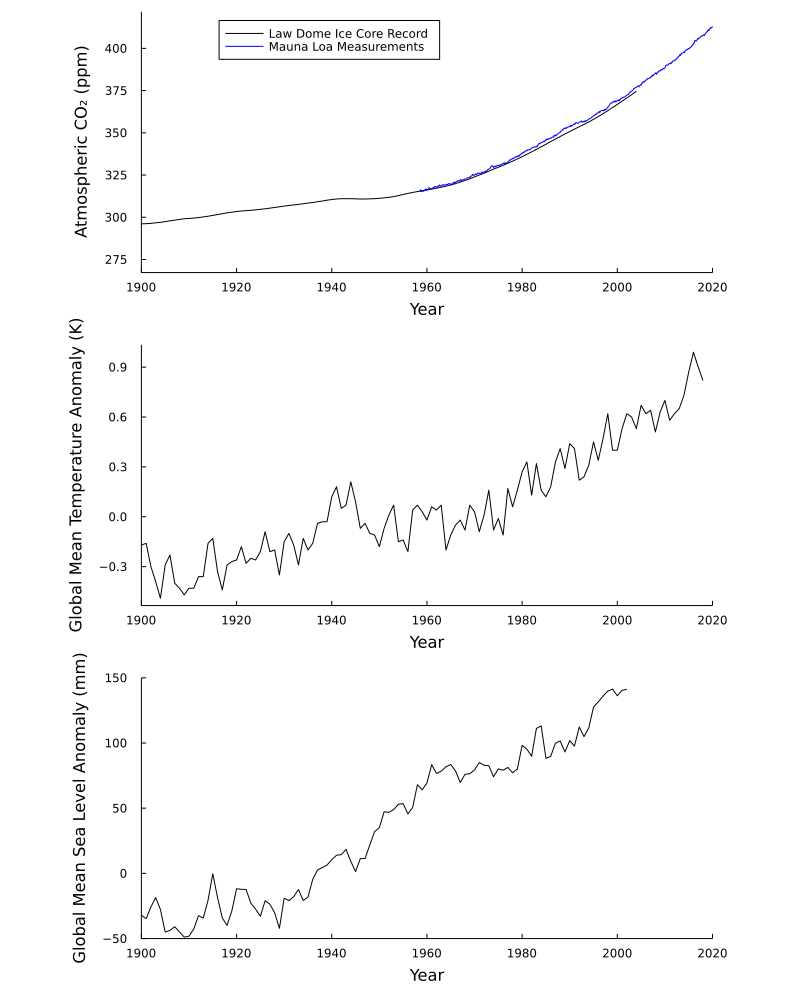
\includegraphics[width=0.75\linewidth]{raes_files/figure-latex/co2tempslr-J1} 

}

\caption{Atmospheric carbon dioxide concentrations (top panel), surface air temperature change (middle panel), and sea level change (bottom panel), between 1900 and ~2015.  All three quantities rise over this period, possibly suggesting a causal relationship between them given a plausible theoretical connection. See text for discussion.}\label{fig:co2tempslr}
\end{figure}

Data covering the last century support this relationship between atmospheric carbon dioxide concentrations, temperature, and sea level (Fig. \ref{fig:co2tempslr}). The curves in the three panels of Figure \ref{fig:co2tempslr} rise together, suggesting that these variables are related.

\begin{center}

\begin{info}
Although correlation does not prove causation, the combination of a clear relationship between variables with a plausible explanation for why they should be related is evidence for causation.

\end{info}


\end{center}

Frequent, accurate measurements of carbon dioxide in the atmosphere began in the late 1950s at Mauna Loa in Hawaii \citep[blue curve in Fig. \ref{fig:co2tempslr}, top panel]{Keeling1976-bc}. These measurements show an annual cycle that represents Northern Hemisphere seasons. Plants lose their leaves or die during the winter, releasing carbon dioxide to the atmosphere. The Northern Hemisphere has much more land, and therefore more plants, than the Southern Hemisphere. Thus, the Northern Hemisphere's seasons largely control the variability in atmospheric carbon dioxide concentrations within any individual year. However, there is a definite upward trend in this curve that is larger than the amplitude of the annual cycle.

Measurements of former atmospheric compositions from bubbles trapped in ice cores allow us to extend the observational record of carbon dioxide concentrations farther back in time \citep[black curve in Fig. \ref{fig:co2tempslr}, top panel]{MacFarling_Meure2006-wa}. As snow falls on the Greenland and Antarctic ice sheets, it traps samples of the atmosphere. Because new snow buries and compresses old snow, the time at which different snow samples fell can be estimated by counting the layers in an ice sheet. The ice core measurements of atmospheric carbon dioxide concentrations are less finely resolved in time than the direct measurements, and therefore don't reflect the annual cycle of CO\textsubscript{2} in the atmosphere. However, the trend of the ice core data is similar to that of the direct observations during the period when they overlap, suggesting that the ice core data are reliable.

Because carbon dioxide mixes readily in the atmosphere, measurements of atmospheric carbon dioxide concentrations at most places on the Earth's surface are relatively representative of the globe as a whole. In contrast, both surface air temperatures and sea levels are measured at widely dispersed stations and must be aggregated to give a global mean value. Global mean temperatures must be estimated from individual weather stations with long records \citep{Hansen2010-wg}; past sea levels are estimated using data from tide gages \citep{Jevrejeva2014-my}. As one might expect, there are various methods for performing this aggregation, and the different methods give somewhat different answers. However, it seems clear that both global mean surface air temperature and global mean sea level are rising.

In this chapter, you'll examine an R script that downloads the data files needed to make the top two panels of Figure \ref{fig:co2tempslr} from the Internet and plots them. You'll then modify the script so that it plots all three panels of Figure \ref{fig:co2tempslr}.

\hypertarget{tutorial}{%
\section{Tutorial}\label{tutorial}}

We'll start by looking at several Web pages that describe the data we'll be using in this exercise. As of May 2015, the various data sets displayed in Figure \ref{fig:co2tempslr} are archived in the following places:

\begin{longtable}[]{@{}lll@{}}
\caption{\label{tab:climatedata} Internet sources of data used in Exercise \#1 and associated references. NOAA, National Oceanic and Atmospheric Administration; DOE CDIAC, United States Department of Energy -- Carbon Dioxide Analysis Center; NASA GISS, National Aeronautics and Space Administration -- Goddard Institute for Space Studies; PSMSL, Permanent Service for Mean Sea Level.}\tabularnewline
\toprule
Data type & Reference & Location on the Web\tabularnewline
\midrule
\endfirsthead
\toprule
Data type & Reference & Location on the Web\tabularnewline
\midrule
\endhead
CO\textsubscript{2}, direct measurements & \citet{Keeling1976-bc} & \href{http://www.esrl.noaa.gov/gmd/ccgg/trends/}{NOAA}\tabularnewline
CO\textsubscript{2}, Law Dome ice core & \citet{MacFarling_Meure2006-wa} & \href{http://cdiac.ornl.gov/trends/co2/modern_co2.html}{DOE CDIAC}\tabularnewline
Surface air temperature change & \citet{Hansen2010-wg} & \href{http://data.giss.nasa.gov/gistemp/}{NASA GISS}\tabularnewline
Sea level anomaly & \citet{Jevrejeva2014-my} & \href{http://www.psmsl.org/products/reconstructions/jevrejevaetal2014.php}{PSMSL}\tabularnewline
\bottomrule
\end{longtable}

Click on the links in the right-hand column of Table \ref{tab:climatedata} and look at the descriptions of the data stored there. Also look for links to the particular data sets mentioned in the Introduction. Some Web pages contain links to multiple data sets; we want the \enquote{\href{ftp://aftp.cmdl.noaa.gov/products/trends/co2/co2_mm_mlo.txt}{Mauna Loa CO\textsubscript{2} monthly mean data},} \href{ftp://ftp.ncdc.noaa.gov/pub/data/paleo/icecore/antarctica/law/law2006.txt}{the Law Dome data} (scroll down to near the bottom of the page), and the \enquote{\href{http://data.giss.nasa.gov/gistemp/tabledata_v3/GLB.Ts+dSST.txt}{global-mean monthly, seasonal, and annual means, 1880-present, updated through most recent month}} of the "Land-Ocean Temperature Index, LOTI.

\hypertarget{downloading-the-data}{%
\subsection{Downloading the Data}\label{downloading-the-data}}

Let's step through how to make the first two panels of the plot above. Notice the liberal use of comments throughout the code; using comments like this is a good way to document your code and help yourself (and others!) interpret it.

\begin{Shaded}
\begin{Highlighting}[]
\CommentTok{# if "data/" does not exist, create it}
\NormalTok{isdir(}\StringTok{"data"}\NormalTok{) || mkdir(}\StringTok{"data"}\NormalTok{); }
\CommentTok{# download files and save in "data"}
\NormalTok{download(}\StringTok{"ftp://aftp.cmdl.noaa.gov/products/trends/co2/co2_mm_mlo.txt"}\NormalTok{, }
    \StringTok{"data/co2_mm_mlo.txt"}\NormalTok{);}
\NormalTok{download(}\StringTok{"ftp://ftp.ncdc.noaa.gov/pub/data/paleo/icecore/antarctica/law/law2006.txt"}\NormalTok{, }
    \StringTok{"data/law2006.txt"}\NormalTok{);}
\NormalTok{download(}\StringTok{"https://data.giss.nasa.gov/gistemp/tabledata_v3/GLB.Ts+dSST.txt"}\NormalTok{, }
    \StringTok{"data/GLB.Ts+dSST.txt"}\NormalTok{);}
\end{Highlighting}
\end{Shaded}

The first line creates a \texttt{data/} directory if one does not already exist. It actually contains a compound command. As discussed in Section \ref{boolean-operators}, \texttt{\textbar{}\textbar{}} is a \emph{short-circuit} or operator. In this context, it first evaluates \texttt{isdir("data")}, which is \texttt{true} if \texttt{data/} exists and is a directory and \texttt{false} if not. If \texttt{isdir("data")} is \texttt{true}, there is no need to continue. If \texttt{data/} does not exist and \texttt{isdir("data")} is \texttt{false}, then it evaluates \texttt{mkdir("data")}, which makes the \texttt{data/} directory. This is a useful alternative in Julia to the following code:

\begin{Shaded}
\begin{Highlighting}[]
\CommentTok{# if "data/" is not a directory, evaluate the rest}
\KeywordTok{if}\NormalTok{ ! isdir(}\StringTok{"data"}\NormalTok{) }
    \CommentTok{# make the "data/" directory}
\NormalTok{    mkdir(}\StringTok{"data"}\NormalTok{) }
\KeywordTok{end}
\end{Highlighting}
\end{Shaded}

The \texttt{download(url,\ location)} commands download files and save them. The \texttt{url} argument is the source for the data, while \texttt{location} is the local path where the file should be saved.

\hypertarget{reading-the-data}{%
\subsection{Reading the Data}\label{reading-the-data}}

Now that we have the files, we need to read the information that they contain into Julia. One of the tricky things with reading files is that you have to know something about how the file is formatted to specify how the code should read it. Open each of the data files using a text editor and examine them. Which files contain \enquote{extra} information at the top or bottom of the file? In each file, which columns contain the information we need?

You may notice that these files are \emph{tab-delimited}, which means that columns are separated using tabs. Ither files may be space-delimited or comma-delimited, also known as comma-separated or CSV files. With this sort of structure, we can read in the files using the \texttt{readdlm()} command, which is short for \enquote{read delimited.} \texttt{readdlm()} is from the \texttt{DelimitedFiles.jl} package, which means we need to load it. \texttt{DelimitedFiles.jl} comes with base Julia, so there's no installation required:

\begin{Shaded}
\begin{Highlighting}[]
\NormalTok{using DelimitedFiles }\CommentTok{# load DelimitedFiles.jl}

\CommentTok{# begin reading in the data}
\CommentTok{#  read Mauna Loa CO2 Data}
\NormalTok{loa_co2data = readdlm(}\StringTok{"data/co2_mm_mlo.txt"}\NormalTok{, skipstart=}\FloatTok{57}\NormalTok{, }
\NormalTok{    header=false);}
\CommentTok{# read Law Dome CO2 Data}
\NormalTok{law_co2data = readdlm(}\StringTok{"data/law2006.txt"}\NormalTok{, skipstart = }\FloatTok{183}\NormalTok{, }
\NormalTok{    header = false)[}\FloatTok{1}\NormalTok{:}\FloatTok{2004}\NormalTok{, :]; }
\end{Highlighting}
\end{Shaded}

In each of the \texttt{readdlm()} commands, the first argument is the file to open. Look at \href{https://docs.julialang.org/en/v1/stdlib/DelimitedFiles/\#Delimited-Files}{the documentation for \texttt{readdlm()}}. We also use two other options: * \texttt{skipstart} skips the specified number of lines from the beginning of the file, which allows us to ignore headings and comments at the beginning of the file; * \texttt{header\ =\ false} tells \texttt{readdlm()} not to interpret the first read line (after the skipped lines) as column headers for the resulting array. We also tell Julia to only keep the first 2004 rows of the Law Dome data (after skipping the first 183 lines of the file). We do this because there is additional information at the bottom of the file that we do not need to keep.

The temperature data file is formatted in blocks, each of which contains about 20 years of data. For that reason, it is much more complicated to read into Julia. The code block below accomplishes this task using a \texttt{for} loop.

\begin{Shaded}
\begin{Highlighting}[]
\CommentTok{# read in temperature data; this requires reading in sections }
\CommentTok{# of the file one at a time}
\CommentTok{# specify the row numbers where each chunk of data begins}
\NormalTok{start_rows = [}\FloatTok{9}\NormalTok{, }\FloatTok{31}\NormalTok{, }\FloatTok{53}\NormalTok{, }\FloatTok{75}\NormalTok{, }\FloatTok{97}\NormalTok{, }\FloatTok{119}\NormalTok{, }\FloatTok{141}\NormalTok{]; }
\CommentTok{# how many rows are in each chunk}
\NormalTok{num_rows = [}\FloatTok{19}\NormalTok{, }\FloatTok{20}\NormalTok{, }\FloatTok{20}\NormalTok{, }\FloatTok{20}\NormalTok{, }\FloatTok{20}\NormalTok{, }\FloatTok{20}\NormalTok{, }\FloatTok{18}\NormalTok{]; }
\CommentTok{# this computes the total amount of data before reading in }
\CommentTok{# each chunk, which we need to index the resulting array}
\NormalTok{cum_num_rows = cumsum(num_rows); }
\CommentTok{# initialize the storage for the temperature data array}
\NormalTok{temp_data = zeros(sum(num_rows), }\FloatTok{20}\NormalTok{); }
\CommentTok{# read in the first chunk}
\NormalTok{temp_data[}\FloatTok{1}\NormalTok{:num_rows[}\FloatTok{1}\NormalTok{], :] = readdlm(}\StringTok{"data/GLB.Ts+dSST.txt"}\NormalTok{, }
\NormalTok{    skipstart = start_rows[}\FloatTok{1}\NormalTok{], header = false)[}\FloatTok{1}\NormalTok{:num_rows[}\FloatTok{1}\NormalTok{], :]; }
\CommentTok{# loop over the remaining chunks and read them in}
\KeywordTok{for}\NormalTok{ i = }\FloatTok{2}\NormalTok{:length(start_rows)}
\NormalTok{    temp_data[(cum_num_rows[i-}\FloatTok{1}\NormalTok{] + }\FloatTok{1}\NormalTok{):cum_num_rows[i], :] = }
\NormalTok{        readdlm(}\StringTok{"data/GLB.Ts+dSST.txt"}\NormalTok{, skipstart = start_rows[i], }
\NormalTok{            header = false)[}\FloatTok{1}\NormalTok{:num_rows[i], :];}
\KeywordTok{end}
\end{Highlighting}
\end{Shaded}

\hypertarget{plotting-the-data}{%
\subsection{Plotting the Data}\label{plotting-the-data}}

Finally, we make the figure. This requires loading the \texttt{Plots.jl} package (see \href{http://docs.juliaplots.org/latest/}{its documentation}), which provides plotting functionality. If this were our first time making plots in Julia, we would need to install \texttt{Plots}, which we would do using \texttt{Pkg}. These lines are commented out in the code below because we've already done this for this book.

\begin{Shaded}
\begin{Highlighting}[]
\CommentTok{## install and load relevant packages}
\CommentTok{# these two lines are commented out as we already have the }
\CommentTok{# `Plots` library installed; if we did not, we would need to }
\CommentTok{# include them}
\CommentTok{# using Pkg}
\CommentTok{# Pkg.add("Plots")}

\CommentTok{# now we load `Plots.jl` as well as the `Plots.Measures` }
\CommentTok{# subpackage, which lets us refer to units like "in" and "mm"}
\NormalTok{using Plots}
\NormalTok{using Plots.Measures}
\CommentTok{# use GR backend; see text discussion}
\NormalTok{gr(); }

\CommentTok{## first plot CO2 data}
\CommentTok{# save the base Law Dome data plot as `p1`}
\NormalTok{p1 = plot(law_co2data[:, }\FloatTok{1}\NormalTok{], law_co2data[:, }\FloatTok{6}\NormalTok{], color=}\StringTok{"black"}\NormalTok{, }
\NormalTok{    label=}\StringTok{"Law Dome Ice Core Record"}\NormalTok{, legend=:top, grid=false);}
\CommentTok{# add the Mauna Loa data on top of the Law Dome data}
\NormalTok{plot!(loa_co2data[:, }\FloatTok{3}\NormalTok{], loa_co2data[:, }\FloatTok{5}\NormalTok{], color=}\StringTok{"blue"}\NormalTok{, }
\NormalTok{    label=}\StringTok{"Mauna Loa Measurements"}\NormalTok{); }
\CommentTok{# label the x-axis}
\NormalTok{xlabel!(}\StringTok{"Year"}\NormalTok{); }
\CommentTok{# we only want to plot data after 1900 even though we have }
\CommentTok{# more from Law Dome}
\NormalTok{xlims!((}\FloatTok{1900}\NormalTok{, }\FloatTok{2020}\NormalTok{)); }
\CommentTok{# label the y-axis}
\NormalTok{ylabel!(}\StringTok{"Atmospheric CO₂ (ppm)"}\NormalTok{); }

\CommentTok{## then plot temperature data}
\CommentTok{# save the base temperature data plot as `p2`}
\NormalTok{p2 = plot(temp_data[:, }\FloatTok{1}\NormalTok{], temp_data[:, }\FloatTok{14}\NormalTok{] / }\FloatTok{100}\NormalTok{, }
\NormalTok{    color=}\StringTok{"black"}\NormalTok{, legend=false, grid=false); }
\NormalTok{xlabel!(}\StringTok{"Year"}\NormalTok{);}
\NormalTok{xlims!((}\FloatTok{1900}\NormalTok{, }\FloatTok{2020}\NormalTok{));}
\NormalTok{ylabel!(}\StringTok{"Global Mean Temperature Anomaly (K)"}\NormalTok{);}

\CommentTok{## combine plots}
\CommentTok{# finally, combine the two plots as two subplot rows}
\NormalTok{plot(p1, p2, layout= (}\FloatTok{2}\NormalTok{, }\FloatTok{1}\NormalTok{), left_margin=}\FloatTok{20}\NormalTok{mm, }
\NormalTok{    right_margin=}\FloatTok{20}\NormalTok{mm); }
\CommentTok{# adjust the size so the final combined plot isn't squished }
\CommentTok{# together}
\NormalTok{plot!(size=(}\FloatTok{800}\NormalTok{, }\FloatTok{600}\NormalTok{)) }
\end{Highlighting}
\end{Shaded}

\begin{figure}

{\centering 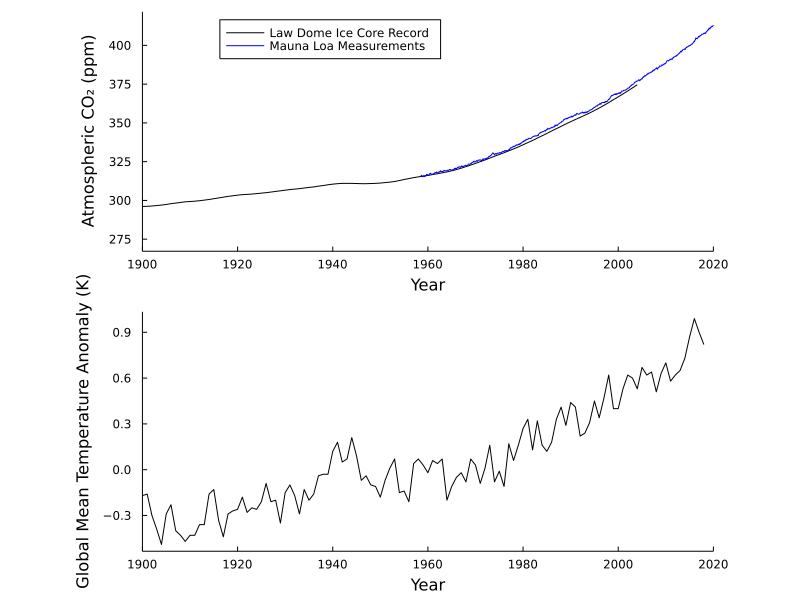
\includegraphics[width=0.75\linewidth]{raes_files/figure-latex/co2temp-J1} 

}

\caption{Plot results after running the code in this chapter. See text for discussion.}\label{fig:co2temp}
\end{figure}

Let's walk through the code preceding Figure \ref{fig:co2temp}. First, \texttt{Plots} \href{http://docs.juliaplots.org/latest/backends/}{uses various backends} to provide varying capabilities. We will use the basic \texttt{GR} backend, so we call \texttt{gr()} after loading \texttt{Plots} to set this up. Next, we plot the Law Dome data using the \texttt{plot()} function. The first argument to \texttt{plot()} contains the x-coordinates of the data; this is the column specifying the year. The second argument are the y-coordinates, which is the sixth column in the data. We can also set the color (\texttt{color=black}) and the legend label (\texttt{label="Law\ Dome\ Ice\ Core\ Record"}), since the atmospheric CO\textsubscript{2} plot will also include the Mauna Loa data. Finally, we set the legend position to be top-center with \texttt{legend=:top} (there are lots of options for legend placement), and turn off the grid corresponding to the axis tick marks with \texttt{grid=false}. Notice that by default, \texttt{plots()} will plot this data as a line, though we could also \href{http://docs.juliaplots.org/latest/tutorial/\#Changing-the-Plotting-Series}{set it to plot the data as points} if desired.

Next, we want to overlay the Mauna Loa data. As discussed earlier, the presence of an exclamation mark after a function name (\texttt{plots!()} as opposed to \texttt{plots()}) means that the function will modify its argument in-place, rather than returning a new variable. This allows us to avoid creating a new set of axes. We color this data blue to distinguish it from the Law Dome data series. We then can add axis labels (using \texttt{xlabel!()} and \texttt{ylabel!()}, which once again modify the current plot rather than creating a new plot object) and change the limits (in this case, we only want to change the x-axis limits to crop the data to post-1900).

Why did we save this plot object in the \texttt{p1} variable? This will allow us to later include it as a subplot in a final combined plot.

The process of creating the second subplot panel, stored as \texttt{p2}, is similar, only we have just the single temperature series, so we never need to make a call to \texttt{plot!()} or set up a legend. In fact, we turn off the legend with \texttt{legend=:false}.

We can now create our combined, two-panel plot with a call to \texttt{plot()}. In this case, we can just specify the two variables which stored our panels, \texttt{p1} and \texttt{p2}, and provide a layout (in the form \texttt{(rows,\ cols)}). It turns out that in this case, doing this cuts off the left and right edges of the plot, so we set a larger margin with \texttt{left\_margin} and \texttt{right\_margin}. We can use intuitive units like \texttt{mm} because we loaded \texttt{Plots.Measures}. Lastly, we modify the size plotting region with \texttt{plot!(size=(800,\ 600))} to spread out the plot to 800 pixels wide by 600 pixels tall and avoid the two panels from running into each other.

What if we wanted to save our figure as a file? To do that, we would use \href{http://docs.juliaplots.org/latest/output/\#savefig-/-format}{\texttt{savefig(filename)}} to save the last plot object in memory to \texttt{filename}. \texttt{savefig()} automatically encodes the plot properly based on the specified file extension.

\hypertarget{exercises}{%
\section{Exercises}\label{exercises}}

\hypertarget{part-1}{%
\subsection*{Part 1}\label{part-1}}


Copy the code from this chapter to a new file. Now, using what you've learned from following the detailed discussion above, modify the new file so that it produces a \texttt{.pdf} file like Figure \ref{fig:co2tempslr}, with three panels. The bottom panel should show the sea level anomalies from \citet{Jevrejeva2014-my}. Specifically, you'll need to add commands to your new file that

\begin{enumerate}
\def\labelenumi{\arabic{enumi}.}
\tightlist
\item
  download the sea level anomaly data from \citet{Jevrejeva2014-my} to your \texttt{data} folder (have a look at Table \ref{tab:climatedata});
\item
  read in this data to a new variable (you might name your new variable \texttt{slr\_data});
\item
  causes the figure to have three panels instead of two;
\item
  plots the sea level anomaly data in the bottom panel;
\item
  adjusts the size of the resulting figure;
\item
  saves the figure to a file.
\end{enumerate}

Make sure that the lower panel of your plot has sensible axis limits in the x and y directions, as well as descriptive labels for the axes (see Fig. \ref{fig:co2tempslr} for an example).

\hypertarget{part-2}{%
\subsection*{Part 2}\label{part-2}}


\begin{enumerate}
\def\labelenumi{\arabic{enumi}.}
\tightlist
\item
  By how much have atmospheric carbon dioxide concentrations, global mean temperatures, and sea levels changed between 1900 and the early part of the present century? Hint: Check Figure \ref{fig:co2tempslr} and/or the figure produced by your updated Julia script.
\item
  How do the changes in atmospheric carbon dioxide concentrations, global mean temperatures, and sea levels between 1900 and 2015 compare to the changes in the same variables between the last ice age (\textasciitilde20,000 years ago) and preindustrial times (around 1850)? Give your results as the changes from Question \#1, above, divided by the changes between the last ice age and the preindustrial period. Note that changes in temperature and sea level were small between 1850 and 1900. You'll need to search the Web for values of these quantities during the last ice age and the preindustrial period. If this exercise is for a class, be sure to give the Internet sources you used in this part of the assignment.
\item
  How do the \emph{rates} of change in atmospheric carbon dioxide concentrations, global mean temperatures, and sea levels between 1900 and 2015 compare to the rates of change in these quantities between the last ice age and preindustrial times? Recall that a rate of change is the change divided by the amount of time over which the change happens.
\end{enumerate}

\hypertarget{normal-distributions-and-the-galton-board}{%
\chapter{Normal distributions and the Galton board}\label{normal-distributions-and-the-galton-board}}

This chapter was written by Patrick J. Applegate and Vivek Srikrishnan.

\hypertarget{learning-objectives-2}{%
\subsection*{Learning objectives}\label{learning-objectives-2}}


After completing this chapter, you should be able to

\begin{itemize}
\tightlist
\item
  describe under what circumstances normal distributions arise
\item
  use quantile-quantile plots to determine whether individual data sets are approximately normal or not
\item
  write simple \texttt{for} loops in Julia
\end{itemize}

\hypertarget{introduction-3}{%
\section{Introduction}\label{introduction-3}}

Suppose that we ask a class of students to walk individually from one end of a field to the other and count the number of steps that they take in order to cover the distance. More than likely, each student will get a somewhat different answer. After each student has paced off the field, we then make a histogram of the number of steps taken by the individual students.

If we were to perform this experiment with a large number of students, the histogram would likely resemble a normal distribution. Normal distributions arise when a large number of measurements are taken of a single quantity, and the individual measurements are affected by random processes that are additive and that can be either positive or negative. The general property that a sufficiently large random sample will be well-described by a normal distribution is called the \href{https://en.wikipedia.org/wiki/Central_limit_theorem}{Central Limit Theorem}, which is foundational in statistics (the details of the Central Limit Theorem are not essential for this book). In our example, the random processes have to do with the varying stride lengths of the students (some take longer strides and some shorter), and counting errors (which are likely to be small and can cause any given student to either over- or underestimate the actual number of paces they took).

A \href{http://mathworld.wolfram.com/GaltonBoard.html}{Galton board} is a physical device that demonstrates this concept (Fig. \ref{fig:galton}). A Galton board has rows of pins arranged in a triangular shape, with each row of pins offset horizontally relative to the rows above and below it. The top row has one pin, the second row has two pins, and so forth.

If a ball is dropped into the Galton board, it falls either to the right or the left when it bounces off the top pin. The ball then falls all the way to the bottom of the board, moving slightly to the right or left as it passes through each row of pins. Bins at the bottom of the board capture the ball and record its final position. If this experiment is repeated with many balls, and if the Galton board includes many rows of pins, the number of balls in each bin resembles a normal distribution (Fig. \ref{fig:galton}).

\begin{figure}
\centering
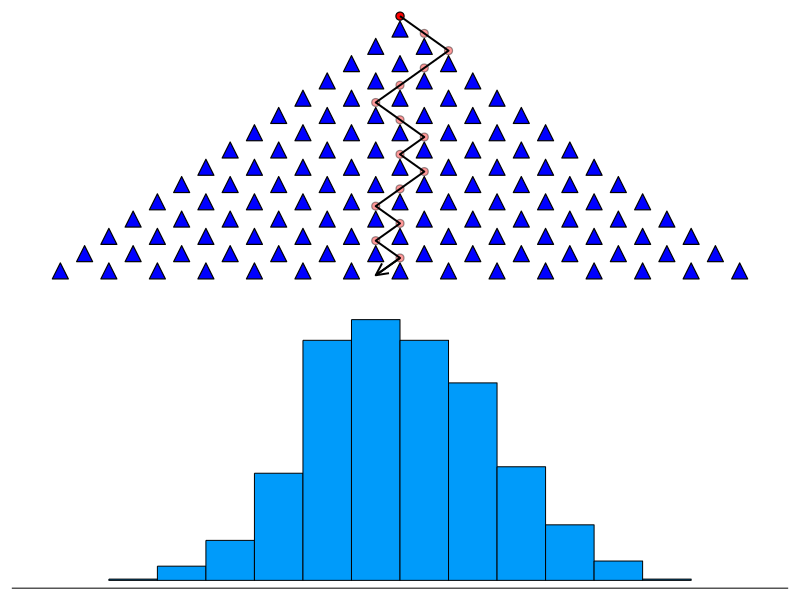
\includegraphics{raes_files/figure-latex/galton-J1.pdf}
\caption{\label{fig:galton}A Galton board simulation with 15 rows of pins. The top panel shows the board and one sample ball trajectory. The bottom panel shows one possible distribution of final ball positions resulting from dropping 1000 balls through the board.}
\end{figure}

In this exercise, you'll experiment with a simple representation of a Galton board in Julia and examine the distributions of final ball positions that it produces. You'll also examine two data sets that can easily be loaded into Julia and see whether they are well described by a normal distribution or not.

\hypertarget{tutorial-1}{%
\section{Tutorial}\label{tutorial-1}}

\hypertarget{writing-our-own-simple-galton-board-script}{%
\subsection{Writing our own simple Galton board script}\label{writing-our-own-simple-galton-board-script}}

Building computer models involves thinking about how to represent the behavior of physical (or chemical, or social) systems in a form that can be understood by a computer. In thinking about how we could represent the Galton board in terms of Julia code, we might start by looking at the diagram of the Galton board in the top part of Figure \ref{fig:galton}. The horizontal spacing between the pins is always the same, but the rows are offset relative to one another; that is, none of the pins in any given row are immediately above or below the pins in the adjacent rows. This offset is exactly half of the horizontal spacing between pins in the same row. Thus, we can imagine that the ball bounces 0.5 distance units to one side whenever it hits a pin.

We first need to specify the number of levels in the Galton board.

\begin{Shaded}
\begin{Highlighting}[]
\NormalTok{levels = }\FloatTok{15}
\end{Highlighting}
\end{Shaded}

\begin{verbatim}
15
\end{verbatim}

We can then represent the path that a single ball takes through the Galton board by randomly sampling how an individual ball bounces as it hits each pin. The Julia package which allows us to do random sampling is \texttt{Random.jl}, which is built into Julia's basic distribution. The function which we call is \texttt{rand()}:

\begin{Shaded}
\begin{Highlighting}[]
\CommentTok{# load the `Random` package}
\NormalTok{using Random}

\CommentTok{# sample}
\NormalTok{path = rand([-}\FloatTok{0.5}\NormalTok{, }\FloatTok{0.5}\NormalTok{], levels)}
\end{Highlighting}
\end{Shaded}

\begin{verbatim}
15-element Vector{Float64}:
  0.5
  0.5
 -0.5
  0.5
 -0.5
  0.5
  0.5
  0.5
 -0.5
 -0.5
 -0.5
 -0.5
  0.5
 -0.5
  0.5
\end{verbatim}

Positive values indicates that the ball bounces to the right; negative values indicate that the ball bounces to the left.

The \texttt{rand()} command generates sequences of values that come from a vector of possibilities supplied in the first argument. The second argument is \texttt{dims}, the dimension of the final sample set. In this case, we are just sampling a single trajectory, so we just need a number of samples equal to \texttt{levels}, which will return a 1-dimensional array.

The bin that the ball lands in is then just

\begin{Shaded}
\begin{Highlighting}[]
\NormalTok{sum(path)}
\end{Highlighting}
\end{Shaded}

\begin{verbatim}
0.5
\end{verbatim}

\hypertarget{doing-things-over-and-over-again-for-loops}{%
\subsection{\texorpdfstring{Doing things over and over again: \texttt{for} loops}{Doing things over and over again: for loops}}\label{doing-things-over-and-over-again-for-loops}}

The commands above tell us about the path that any single ball takes through the Galton board, as well as the bin it finally lands in. But, suppose we want to write a piece of R code that performs this calculation for many balls and gives us a histogram of the bins that they land in. How could we do that?

Most, perhaps all, programming languages include a method for carrying out a set of instructions a fixed number of times. In most programming languages, including Julia, this method is called a \texttt{for} loop. The syntax of \texttt{for} loops in Julia looks like this:

\begin{Shaded}
\begin{Highlighting}[]
\CommentTok{# set the number of times the loop should be evaluated; }
\CommentTok{# this is not part of the for loop syntax}
\NormalTok{neval = }\FloatTok{3}\NormalTok{; }
\KeywordTok{for}\NormalTok{ i = }\FloatTok{1}\NormalTok{:neval}
  \CommentTok{# instructions to be repeated go here }
\NormalTok{  println(i^}\FloatTok{2}\NormalTok{)}
\KeywordTok{end} 
\end{Highlighting}
\end{Shaded}

\begin{verbatim}
1
4
9
\end{verbatim}

\begin{Shaded}
\begin{Highlighting}[]
\CommentTok{# note the end; this is required to tell Julia where the }
\CommentTok{# loop instructions end!}
\end{Highlighting}
\end{Shaded}

This sample \texttt{for} loop is not very exciting: it simply \texttt{println()}s the square of the \emph{index variable} \texttt{i} during each iteration of the indented commands (between \texttt{for} and \texttt{end}).

In \enquote{real} \texttt{for} loops, the name of the index variable, the vector of values that the index variable can take (here \texttt{1:neval}), and the evaluated instructions can be more complex. In particular, there can be more than one line of instructions evaluated. In Julia, you can also iterate over arbitrary collections, such as arrays, not just sequences of index variables.

We usually will want to create a variable that will store the results from the commands carried out within the \texttt{for} loop. The following block of code generates and \texttt{print()}s the first five \href{https://en.wikipedia.org/wiki/Fibonacci_number}{Fibonacci numbers}:

\begin{Shaded}
\begin{Highlighting}[]
\NormalTok{neval = }\FloatTok{5} 
\end{Highlighting}
\end{Shaded}

\begin{verbatim}
5
\end{verbatim}

\begin{Shaded}
\begin{Highlighting}[]
 \CommentTok{# make a vector of `neval` zeroes, which will store the output}
\NormalTok{fibonacci = zeros(neval)}
\end{Highlighting}
\end{Shaded}

\begin{verbatim}
5-element Vector{Float64}:
 0.0
 0.0
 0.0
 0.0
 0.0
\end{verbatim}

\begin{Shaded}
\begin{Highlighting}[]
\KeywordTok{for}\NormalTok{ i = }\FloatTok{3}\NormalTok{:neval}
  \CommentTok{# stores the sum of the preceding two elements of `fibonacci` }
  \CommentTok{# in the ith element of `fibonacci`}
\NormalTok{  fibonacci[i] = sum(fibonacci[i-}\FloatTok{2}\NormalTok{:i-}\FloatTok{1}\NormalTok{])}
\KeywordTok{end}
\NormalTok{println(fibonacci)}
\end{Highlighting}
\end{Shaded}

\begin{verbatim}
[0.0, 0.0, 0.0, 0.0, 0.0]
\end{verbatim}

In general, it's good practice to pre-allocate storage for the output of \texttt{for} loops as we did by defining the \texttt{fibonacci} array. If we were to just start with the initial two Fibonacci numbers and add to the length of the array at each iteration, this would slow down the program's execution due to the need to assign new memory to the resulting array every time it grew. This might not be noticeable for the code block above due to the small number of evaluations, but it will be for more complex code.

In the Exercise below, you'll put together the information above to write your own script for making histograms of the outcomes from a Galton board. First, though, let's examine how we determine whether a particular data set is normal or not.

\hypertarget{normal-or-not-normal-generating-and-interpreting-quantile-quantile-plots}{%
\subsection{Normal or not normal?: Generating and interpreting quantile-quantile plots}\label{normal-or-not-normal-generating-and-interpreting-quantile-quantile-plots}}

It can be tempting to assume that a particular process gives normally-distributed output, or that data are normally distributed; however, assuming normality when it isn't present can lead to large errors. How can we check individual data sets for normality?

One robust and simple, but approximate, test for normality involves making a \href{https://en.wikipedia.org/wiki/Q-Q_plot}{quantile-quantile (Q-Q) plot}. The details of how Q-Q plots work aren't important for our purposes here. However, if data are drawn from a normal distribution, they will lie on a line connecting the first and third quartiles of the data when drawn on an appropriately-constructed Q-Q plot. The \href{https://github.com/JuliaPlots/StatsPlots.jl}{\texttt{StatsPlots.jl} package} makes drawing Q-Q plots easy.

To see how this looks, let's examine samples from different distributions. We can do this using the \texttt{Distributions.jl} package, which lets us specify distributions to sample from. We can then use \texttt{rand()} from the

For example, the following block of code generates 100 random numbers from a normal distribution, makes a Q-Q plot from them, and draws a 1:1 line on the plot:

\begin{Shaded}
\begin{Highlighting}[]
\CommentTok{# load the packages we will use}
\NormalTok{using Distributions}
\NormalTok{using Random}
\NormalTok{using StatsPlots}

\CommentTok{# specify the normal distribution with mean = 0 }
\CommentTok{# snd standard deviation = 1, which are the default choices}
\NormalTok{normal_distribution = Normal();}
\CommentTok{# draw 100 samples}
\NormalTok{normal_samples = rand(normal_distribution, }\FloatTok{100}\NormalTok{);}
\CommentTok{# make the Q-Q plot}
\NormalTok{qqplot(Normal(), normal_samples) }
\end{Highlighting}
\end{Shaded}

\begin{figure}
\centering
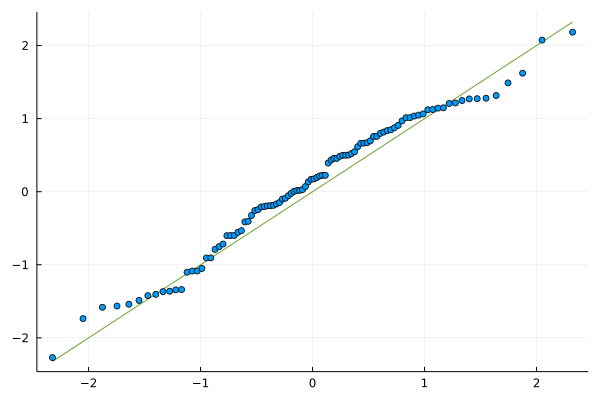
\includegraphics{raes_files/figure-latex/qqnormal-J1.pdf}
\caption{\label{fig:qqnormal}A Q-Q plot showing 100 normally-distributed random values. The points, which represent the random values, lie approximately on the line, showing that their distribution could be treated as a normal distribution.}
\end{figure}

If we have a data set, we might not know what the parameters of the normal distribution are for the comparison (in this case, they were just the defaults). One strategy is to use the sample mean and standard deviation, which can be obtained with \texttt{mean()} and \texttt{std()} (this is justified by the Central Limit Theorem).

Let's see what a Q-Q plot might look like if we draw samples from a distribution that isn't normal. We will sample from a \href{https://en.wikipedia.org/wiki/Cauchy_distribution}{Cauchy distribution}, which is a distribution which has a higher probability of extreme values than a normal distribution.

\begin{Shaded}
\begin{Highlighting}[]
\CommentTok{# specify the default Cauchy distribution }
\NormalTok{cauchy_distribution = Cauchy();}
\CommentTok{# draw 100 samples}
\NormalTok{cauchy_samples = rand(cauchy_distribution, }\FloatTok{100}\NormalTok{);}
\CommentTok{# make the Q-Q plot}
\NormalTok{qqplot(Normal(), cauchy_samples) }
\end{Highlighting}
\end{Shaded}

\begin{figure}
\centering
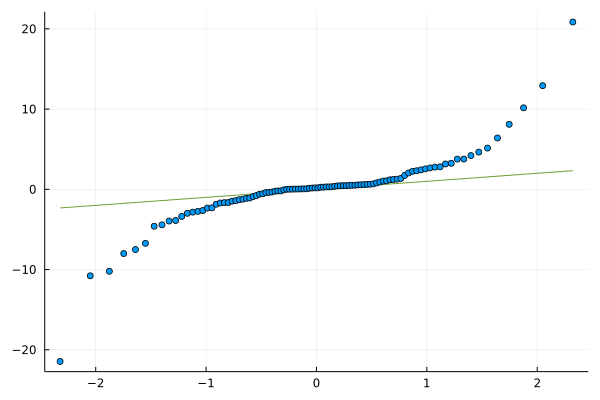
\includegraphics{raes_files/figure-latex/qqcauchy-J1.pdf}
\caption{\label{fig:qqcauchy}A Q-Q plot showing 100 Cauchy-distributed random values. The points, which represent the random values, do not lie on the line for the majority of the plot. In this case, it could be dangerous to assume that the data were normally-distributed.}
\end{figure}

Unlike in Figure \ref{fig:qqnormal}, the points in Figure \ref{fig:qqcauchy} are generally not along the line, which should suggest to use that the data are not normally distributed. On the left side of the Q-Q plot, the points are well below the line, and on the right side, they are well above it. This actually gives us more information about how the sample deviates from being normally distributed! The fact that the left side is below the line shows us that the distribution is \enquote{fatter} below the mean than a normal distribution, or that its left tail is heavier than that of a normal distribution. This is because a normal distribution's samples are more limited in range than the samples from the Cauchy distribution. This means that it is more likely to see large negative values in this sample than we would expect from a normal sample. Similarly, the right side being above the line shows us that large positive values are more present than we would expect from a normal sample, and the right tail is fatter than a normal distribution's. If the points and the line had the opposite relationship, we could conclude that the sample had thinner tails, and was more concentrated, than would be expected from a normal distribution. And if we had a mixed situation, that would suggest to us that our sample was more skewed to one side or the other.

\hypertarget{exercises-1}{%
\section{Exercises}\label{exercises-1}}

\hypertarget{part-1-1}{%
\subsection*{Part 1}\label{part-1-1}}


Based on the information presented in this chapter, write a Julia script that

\begin{enumerate}
\def\labelenumi{\arabic{enumi}.}
\tightlist
\item
  sets values for the number of balls to drop and the number of rows of pins in the Galton board (you might use the variable names \texttt{nballs} and \texttt{levels})
\item
  creates a vector \texttt{output} that contains a number of elements equal to \texttt{nballs}; these elements can be populated with \texttt{0}s or \texttt{nothing}s to start;
\item
  uses a \texttt{for} loop that
\end{enumerate}

\begin{itemize}
\tightlist
\item
  runs through values of the index variable \texttt{i} from \texttt{1:nballs},
\item
  determines which bin of the Galton board each ball lands in, and
\item
  stores these values in the different elements of \texttt{output}
\end{itemize}

\begin{enumerate}
\def\labelenumi{\arabic{enumi}.}
\setcounter{enumi}{3}
\tightlist
\item
  makes a histogram of \texttt{output}. The code block below shows one way of carrying out this step.
\end{enumerate}

\begin{Shaded}
\begin{Highlighting}[]
\CommentTok{# Make a histogram of the results.}
\NormalTok{using Plots}
\NormalTok{gr();}
\NormalTok{histogram(output, xlabel = }\StringTok{"Bin"}\NormalTok{, ylabel = }\StringTok{"Count"}\NormalTok{, }
\NormalTok{  legend=:false)}
\end{Highlighting}
\end{Shaded}

Set the number of rows of pins in your Galton board R script to 10. Also set the number of balls to drop to a low value, say 10 to begin. + How does the histogram change as you repeatedly run the script? + What is the smallest number of balls that you can drop that gives more or less the same histogram each time you run the script, for 10 rows of pins?

\begin{center}

\begin{info}
We could also do this problem differently by sampling all the trajectories for all the balls simultaneously. We would do this by specifying a tuple for the \texttt{dims} argument of \texttt{rand()}. If we wanted to sample \texttt{nballs} ball paths at once, we could set \texttt{dims=(nballs,\ levels)} and the result will be formatted as an array with \texttt{nballs} rows and \texttt{levels} columns. We would then iterate over the array and sum to get the final positions for each of the \texttt{nballs}.

\end{info}


\end{center}

\hypertarget{part-2-1}{%
\subsection*{Part 2}\label{part-2-1}}


Add commands to your Julia script so that it also generates a Q-Q plot for the results in \texttt{output}.

Recall from the discussion above that a Galton board only gives an approximately-normal distribution if both the number of balls that are dropped and the number of bins are large. Leaving the number of rows of pins at 10, increase the number of balls to a large value like 10\textsuperscript{4} (in code, that would be just \texttt{10\^{}4}). Confirm that the \texttt{output} under these circumstances is not normally distributed. How large does the number of rows of pins have to be to get approximately-normal results?

\hypertarget{part-3}{%
\subsection*{Part 3}\label{part-3}}


Generate Q-Q plots for two commonly-used data sets,

\begin{itemize}
\tightlist
\item
  the \href{https://www.rdocumentation.org/packages/datasets/versions/3.6.2/topics/faithful}{waiting time between Old Faithful eruptions}, and
\item
  the \href{https://www.rdocumentation.org/packages/datasets/versions/3.6.2/topics/iris}{sepal length of setosa irises on the Gaspe Peninsula}.
\end{itemize}

\begin{enumerate}
\def\labelenumi{\arabic{enumi}.}
\tightlist
\item
  Install and load the \texttt{RDatasets} package.
\item
  Load the Old Faithful (\texttt{dataset("datasets",\ "faithful"){[}:,\ 2{]}}) and iris sepal (\texttt{dataset("datasets",\ "iris3"){[}:,\ 1,\ 1{]}}) datasets.
\item
  Generate your Q-Q plots.
\end{enumerate}

Which of these datasets is approximately normally distributed, and which is not? How can you tell?

\backmatter

\renewcommand\bibname{References}
  \bibliography{bibliography/bibliography.bib}

\end{document}
